% Appendix Template

\chapter{Converting dataset from CSV to Graph} % Main appendix title

\label{AppendixB} % Change X to a consecutive letter; for referencing this appendix elsewhere, use \ref{AppendixX}

\lhead{Appendix B. \emph{Converting dataset from CSV to Graph}}
Currently, the dataset is in a CSV format which needs to be converted into a Graph format for which we can then feed into the GNN model.
To keep things simple for the baseline model, we model all the employees and EACH mail as a node in a heterogeneous graph containing two different node types. After this we create an edge between the following pairs:

\begin{itemize}[noitemsep,topsep=0pt]
    \item (sender, message)
    \item (receiver, message)
    \item (sender,receiver)
\end{itemize}

Mail node contains an attribute called reply which contains 0 or 1 based on whether this particular message received a reply or not.
The final graph created is an undirected heterogeneous multi-graph since the nodes are connected to multiple nodes.

\begin{center}
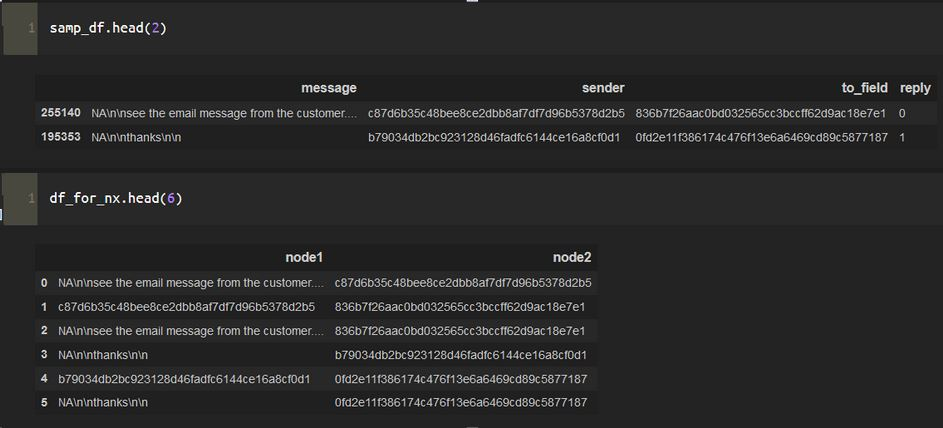
\includegraphics[scale=0.75]{Appendices/image1_graph.JPG}
\end{center}

To create the graph from CSV, the node pairs mentioned earlier need to be created. The code above shows the original dataframe and the new dataframe used to create the graph. They both contain the same data, just in different format
\begin{center}
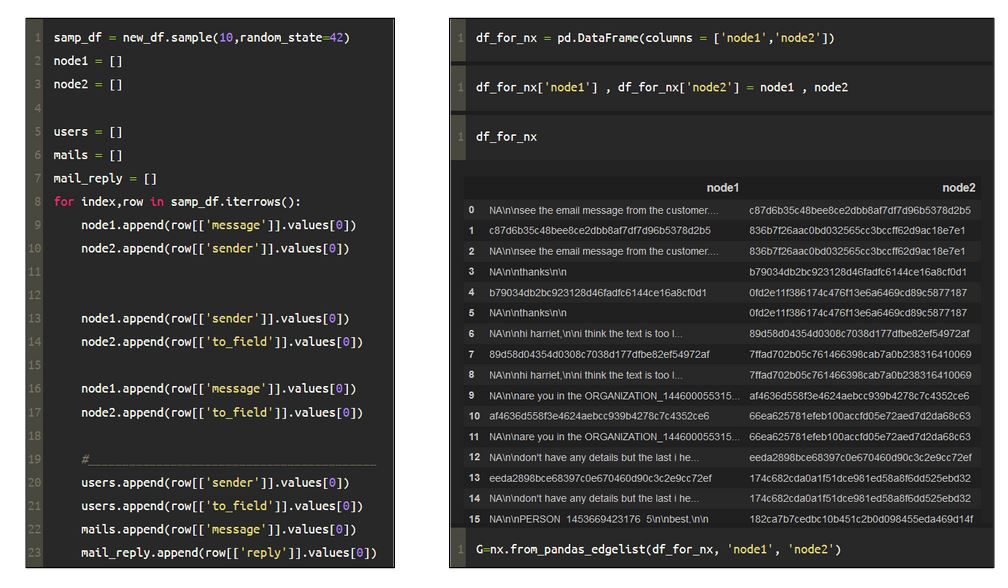
\includegraphics[scale=0.75]{Appendices/image2_graph.JPG}
\end{center}

Using this code, a networkx graph is created which can be used with a Graph Machine Learning Library.

\begin{center}
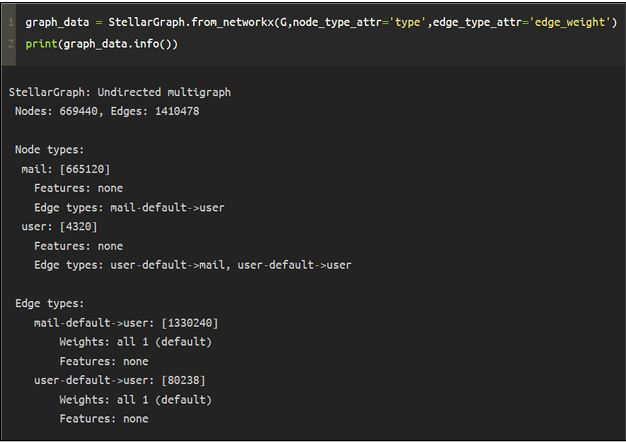
\includegraphics[scale=0.75]{Appendices/image3_graph.JPG}
\end{center}


